\chapter{Methodology}
\label{ch:method}

\section{Data Collection and Preprocessing}

\subsection{Data Sources}

\begin{itemize}
    \item \textbf{Database of East African Mesoscale Convective Systems (MCSs)}
    \begin{itemize}
        \item File: \texttt{East\_Africa\_tracked\_MCSs\_2014\_2019\_longer\_than\_3\_hours.csv}
        \item Contains 27,982 storms longer than 3 hours, with all storm centroids along the track within (3--15N, 34--52E)
    \end{itemize}
    \item \textbf{ERA5 Data}
    \begin{itemize}
        \item ERA5 data for 31--53E, 2--16N region for 2014--2019, totalling 27 GB
        \item The ERA5 area is slightly wider by a few grid points to account for edge cases in the database and for calculating gradients
    \end{itemize}
\end{itemize}

\subsection{Feature Engineering}

\begin{itemize}
    \item cleaning
    \item means over 400km
    \item domain means
    \item storm aggregate features
\end{itemize}

\subsection{Feature Selection}

\begin{itemize}
    \item highly correlated features removed
    \item data leakage prevention measures implemented
    \begin{itemize}
        \item related features
        \item features with info from future
    \end{itemize}
\end{itemize}

\section{Modelling Approach}

\subsection{XGBoost}

\begin{itemize}
    \item general explanation of XGBoost
    \item advantages of using XGBoost for this task
\end{itemize}

\subsection{Hyperparameter Tuning}

\begin{itemize}
    \item Weights \& Biases sweep with Bayesian optimization
    \item cross-validation for training on each trial
\end{itemize}

\subsection{Performance Comparison}

\begin{itemize}
    \item compare performance metrics (e.g., accuracy, F1 score) across different models
    \item analyse discrepancies in performance across different feature sets
    \item analyse average performance across different regions and time periods? \todo{if no time, this is for future work section}
\end{itemize}

\section{Model Explainability}
\todo{copied from background; will need to be adapted}

\acrfull{xai} is an emerging field focused on developing methods and techniques to make the decision-making processes of \acrshort{ml} solutions more transparent and interpretable. Approaches in this field take a variety of forms, including inherently interpretable models and post-hoc explanation methods. A summary of \acrshort{xai} taxonomy is given in Figure \ref{fig:xai-taxonomy}.

\begin{figure}[ht]
    \centering
    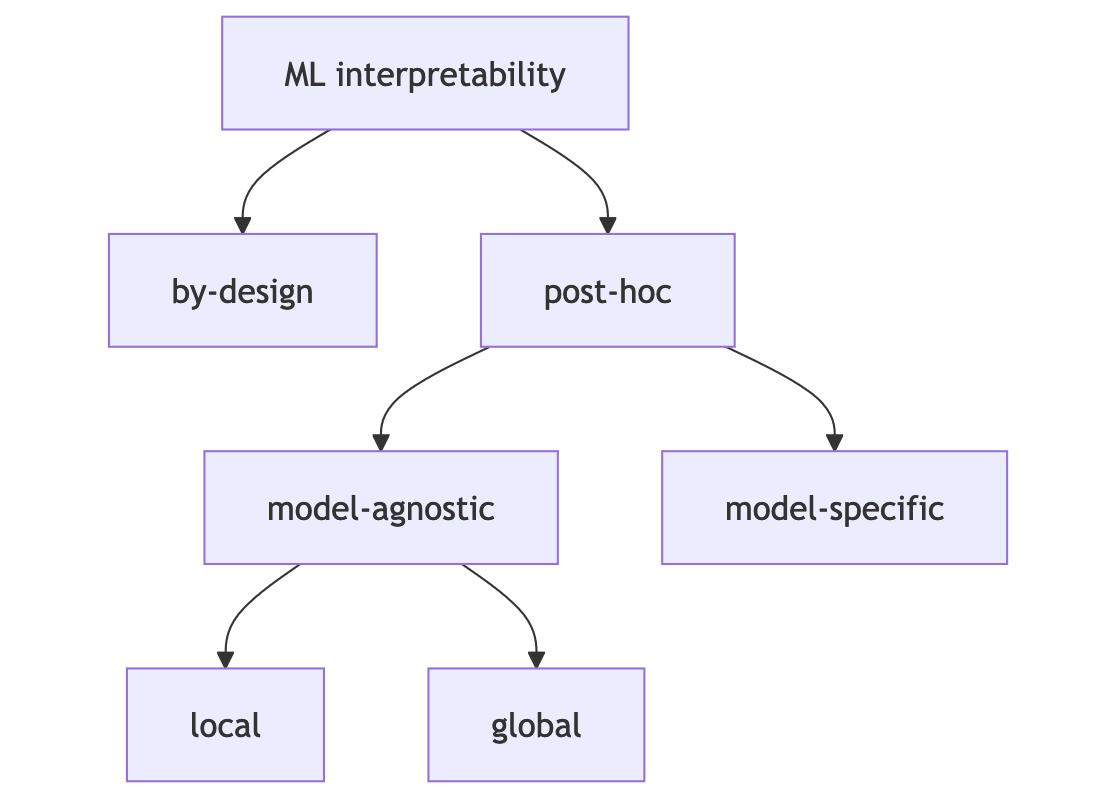
\includegraphics[width=0.8\textwidth]{../figures/static/xai-taxonomy.jpg}
    \caption{\acrshort{xai} Taxonomy \citep{Molnar2025}}
    \label{fig:xai-taxonomy}
\end{figure}

Inherently interpretable models are designed to be transparent by construction, often using simpler architectures or feature-based approaches that allow for direct interpretation of the relationship between inputs and outputs. Examples include linear regression, decision trees, and rule-based systems. A clear disadvantage is that these simpler models may sacrifice some predictive performance compared to more complex ones like \acrfull{dnn}. \acrshort{piml} could also be considered a part of this landscape, as it aims to integrate existing physical knowledge into architectures and training processes to enhance forecast accuracy and credibility. Post-hoc explanation methods, on the other hand, are applied to models after training to partially interpret their behaviour. Model-specific post-hoc methods directly leverage the learned structure of the model. For example, great strides have been made in pinning the internal embeddings and attention mechanisms of transformer models to real-world entities and concepts \citep{Lin2023}. Notably for this research, model-agnostic methods are predominantly designed to make no assumptions about a model's underlying architecture. These methods can then be broadly categorised into local and global explanations. Local explanations focus on providing insights into model behaviour around a given input. In contrast, global explanations aim to provide an overall understanding of the model's behaviour for any input. For local explanations, counterfactual analysis has gained traction, especially for classification tasks, where the model's local decision boundary can be more interactively explored through slight perturbations of the a given input \citep{Mothilal2019}. \acrfull{shap} is both applicable for local and global explanations and will be used extensively throughout this research. As such, a brief overview of the approach follows.

\subsection{Shapley Additive Explanations}

After its popularisation via \cite{Lundberg2017} and the accompanying \texttt{shap} \texttt{python} library, \acrfull{shap} has emerged as one of the most prominent frameworks for post-hoc explainability. This is achieved through the application of coalitional game theory where the algorithm approximates a fair distribution of "payout", in this case a fraction of the model's prediction, among the input features based on their individual contributions to the prediction \citep{Shapley1953}. Formally, the Shapley value for a feature is calculated via the average marginal contribution of that feature across all possible coalitions of features weighted by the probability of the coalition, where a coalition is a subset of features, and the marginal contribution of a feature to a coalition is the difference in the model's prediction when that feature is included versus when it is excluded. This process ensures that each feature's contribution is fairly evaluated by accounting for its interactions with other features. The result is a set of Shapley values for each feature and model output, which can then be used to interpret the model's predictions locally, by highlighting the most influential features for a single output, or globally, by aggregating the Shapley values across multiple predictions to identify overall feature importance.

In practice, this algorithm experiences a \gls{combinatorialexplosion} as features increase, thus, various approximations and optimisations have been developed to make it feasible for larger datasets. For example, \cite{Lundberg2017} present a kernel-based method which operates on the assumption that not all coalitions are equally important in quantifying a features marginal contribution. The application of Shapley values for explaining \acrshort{ml} models was first proposed by \cite{trumbelj2011}, but \cite{Lundberg2017} key contribution was the introduction of an additive feature attribution model, which allows for efficient approximation using a linear model. This approach assumes that the prediction can be expressed as a sum of the feature contributions, making it easier to interpret and visualise. The \texttt{shap} library implements both model-specific and agnostic methods using this framework and provides various tools for visualising Shapley values and their impact on individual predictions and overall model performance.

\begin{itemize}
    \item use shap values to identify key features driving model predictions
\end{itemize}

\subsection{Geographic and Temporal Distribution of Feature Importance}

\begin{itemize}
    \item find highest correlation (or other relation measure) of shap values to lon, lat, eat hours, and date angle to analyse feature importance across different regions and time periods
\end{itemize}